\documentclass[14pt,a4paper,russian]{scrartcl}
\usepackage[utf8]{inputenc} % кодировка
\usepackage[T2A]{fontenc}
\usepackage[russian,english]{babel}
\usepackage{mathtext}
\usepackage{indentfirst}    % красная строка для первого параграфа
\usepackage{misccorr}   % настройки для российской полиграфии
\usepackage{graphicx}
\usepackage{textcomp}
\usepackage{caption}
% \usepackage{times}
% \usepackage{amsmath}    % математическая нотация
% \renewcommand{\rmdefault}{ftm}
\usepackage{lastpage}

\usepackage{setspace} 
\usepackage{fancybox,fancyhdr}
% \usepackage[utf8]{inputenc}
% \usepackage[russian,english]{babel}
% \usepackage[T2A]{fontenc}
% \usepackage{indentfirst}w
\usepackage{amsmath,amssymb}
\usepackage[includefoot, heightrounded]{geometry}   % поля
\geometry{left=30mm}
\geometry{right=20mm}
\geometry{top=20mm}
\geometry{bottom=10mm}
\begin{document}
% \pagestyle{fancy}
\fancyhead[R]{Кочнов Андрей, ИУ1-62}
% \renewcommand{\onlyinsubfile}[1]{}
% \renewcommand{\notinsubfile}[1]{#1}
\captionsetup[table]{name=Таблица}
\captionsetup[figure]{name=Рисунок}

\begin{table}[h]
    \begin{center}
        \begin{tabular}{p{0.6\linewidth}p{0.4\linewidth}}
            Заготовка РПЗ по ОКП&Кочнов Андрей, ИУ1-62\\
            \hline
        \end{tabular}
    \end{center}
\end{table}
\section*{Техническое задание}
\subsubsection*{Тема: привод следящей системы (задание №3)}
Разработать конструкцию привода следящей системы по предложенной схеме
в соответствии с заданным вариантом.
\begin{table}[h]
    \begin{center}
        \begin{tabular}{|p{0.6\linewidth}|p{0.4\linewidth}|}
            \hline
            Вариант &   2 \\
            \hline
            Скорость вращения выходного вала \( \omega,\ c^{-1} \) & 5 \\
            \hline
            Ускорение вращения выходного вала \( \epsilon,\ c^{-2} \) & 36 \\
            % 0.5 & 360 & 4 & 110 & 0.022 & 0.04 \\
            \hline
            Момент инерции нагрузки \( J,\ \text{кгм}^2 \) & 0,015\\
            \hline
            Угол поворота выходного вала \( \phi \) & 120\\
            \hline
            Присоединительный диаметр \( d,\ \text{мм} \) & 50 \\
            \hline
            Тип потенциометра & ПТП или ППМЛ - выбирается самостоятельно
                с соответствующим обоснованием \\
            \hline
            Тип электродвигателя & Выбирать из серий ДИД, ДГ \\
            \hline
        \end{tabular}
        \caption{Исходные данные для расчёта}\label{tab:source}
    \end{center}
\end{table}

\newcommand{\Mnom}{M_{\text{ном}}}
\newcommand{\Mp}{M_{\text{п}}}
\newcommand{\nn}{n_{\text{ном}}}
\newcommand{\nv}{n_{\text{вых}}}

\setcounter{section}{1}
\section*{Расчётная часть}
\subsection{Предварительный расчёт электродвигателя}
    Сначала вычислим момент нагрузки на выходном валу:
    \[ M = J\epsilon = 0,015\cdot36 = 540\ \text{Нмм}\]
    Затем вычислим минимально возможную мощность двигателя, используя формулу
    \[ N = \xi\frac{M\omega}{\eta_p}. \]
    Приняв запас прочности \( \xi=1,1 \), а оценочный КПД редуктора \( \eta_p=0.8 \),
    получим \( N=3.71\ \text{Вт} \).

    Предварительно выберем двигатель ДГ-5ТА:
    \begin{table}[h!]
        \begin{center}
            \begin{tabular}{|p{0.6\linewidth}|p{0.4\linewidth}|}
                \hline
                Мощность \( N \), Вт & 5 \\
                \hline
                Номинальный момент \( \Mnom \), Нмм & 10 \\
                \hline
                Пусковой момент \( \Mp \), Нмм &    22 \\
                \hline
                Скорость вращения вала \( \nn \), об\( \backslash \)мин     & 6000 \\
                \hline
                Момент инерции ротора \( J_p \), \( \text{кгм}^2 \) & 4E-7 \\
                \hline
                Напряжение питания U, В & 36 \\
                \hline
            \end{tabular}
            \caption{Параметры двигателя}\label{tab:engine}
        \end{center}
    \end{table}

    \subsection{Кинематический и вспомогательный силовой расчёты}
    \subsubsection{Определение общего передаточного отношения}
        Вычислим общее передаточное отношение редуктора по формуле 
         \[ i_0 = \frac{\nn}{\nv}. \]
         Скорость вращения выходного вала находим по формуле 
          \[ \nv = \frac{30\omega}{\pi}. \]
         В результате получаем
          \[ i_0 = \frac{\nn\pi}{30\omega} = \frac{6000\cdot3,14}{30\cdot5} = 126\]
    
    \subsubsection{Определение числа ступеней}
        Число ступеней будем определять исходя из критериев минимизации
        момента инерции и габаритов, используя обьединённую формулу:
         \[ n = \frac{3+1,85}{2}\cdot\lg\ i0 \approx 5 \]
        Таким образом, редуктор будет иметь 5 ступеней.
    
    \subsubsection{Определение передаточных отношений каждой ступени}
        Распределение будет производить исходя из критерия минимизации
        момента инерции.
        Сперва вычислим среднее геометрические передаточное отношение [1]:
        \newcommand{\iavr}{i_{\text{ср}}}
         \[ \iavr = \sqrt[n]{i_0} = \sqrt[5]{126} = 2.63 \]
        Затем рассчитаем непосредственно значения передаточного отношения для каждой ступени:
         \[ i_1 = \sqrt[4]{2\iavr} = 1.51 \]
        \[ i_2 = \sqrt{\iavr} = 1.62 \]
        \[ i_3 = \iavr = 2.63 \]
        \[ i_4 = \frac{\iavr^2}{i_2} = 4.27 \]
        \[ i_5 = \frac{\iavr^2}{i_1} = 4.57\]
    
    \subsubsection{Определение числа зубьев зубчатых колёс}
        Для подбора числа зубьев для шестерней имеет смысл брать минимальные из стандартного ряда,
        однако в процессе разработки конструкции делаются поправки исходя из необходимых
        минимальных расстояний между валами.
        Для колёс рассчитаем числа зубьев \( z_i \), воспользовавшись формулой
        \[ z_i = z_{i-1}i_j, \]
        где \( z_{i-1} \) - число зубьев соответствующей шестерни, а \( i_j \) - 
        передаточное отношение данной пары.
        
        По итогам расчётов получаем следущие значения:
        \begin{table}[h!]
            \begin{center}
                \begin{tabular}{p{0.13\linewidth}p{0.23\linewidth}p{0.2\linewidth}}
                    \hline
                    Номер ступени & Z для шестерни & Z для колеса \\
                    \hline
                    1   &   25 & 38 \\
                    % \hline
                    2   &   25 & 38 \\
                    % \hline
                    3   &   25 & 71 \\
                    % \hline
                    4   &   25 & 106 \\
                    % \hline
                    5   &   36 & 160 \\
                    \hline
                \end{tabular}
                \caption{Значения числа зубьев для зубчатых колёс}\label{tab:gears_z}
            \end{center}
        \end{table}
        
        В связи с тем, что стандартный ряд числа зубьев весьма дискретен, 
        результирующее передаточное отношение редуктора может отличаться от начального.
        Вычислим погрешность:
        \[ \Delta i = \frac{|i_0 - i_{\text{фактич.}}|}{i_0} =  
            \frac{|126-123.65|}{126} = 0.019\]
        
        Результат вполне удовлетворяет требования точности.
        
    \subsubsection{Приведение моментов к валам}
        Для расчёта дальнейших параметров зубчатых колёс необходимо найти крутящие моменты,
        действующие на каждом из валов редуктора. Для этого воспользуемся формулой [1]
        \[ M_p = \frac{M_q}{i_{p-q}\eta_{pq}\eta_n}, \]
        где \( M_p, M_q \) - моменты нагрузки на p-м и q-м валах,
            \( i_{p-q} \) - передаточное отношение между валами,
            \( \eta_{pq},\ \eta_n \) - КПД зацепления (для цилиндрической 0,98) и подшипников (0,99)\par
        
        По итогам вычислений получаем следующий результат (\( M_0 \) - вал двигателя):
        \begin{table}[h!]
            \begin{center}
                \begin{tabular}{p{0.2\linewidth}p{0.1\linewidth}p{0.1\linewidth}p{0.1\linewidth}p{0.1\linewidth}p{0.1\linewidth}p{0.1\linewidth}}
                    \hline
                    Номер вала, p & I & II & III & IV & V & VI \\
                    \hline
                    \( M_p \), Нмм & 5 & 7.33 & 11.52 & 29.4 & 121.79 & 540 \\
                    \hline
                \end{tabular}
                \caption{Оценочные значения моментов на валах}\label{tab:moments__shaft_estimate}
            \end{center}
        \end{table}

        Заметим, что \( M_0=5 \) Н, что в 2 раза меньше значения номинального момента двигателя 10 Н,
        т.е. имеем большой запас по моменту двигателя.

    \subsubsection{Определение модуля зацепления}
        Модуль зацепления берётся по результатам расчётов зубьев на контактную и
        изгибную прочность. Расчёт на изгибную прочность проводится по наиболее нагруженной ступени в целях
        сокращения математических выкладок. Основная его формула [1]
        \[ m \geq K_m\sqrt[3]{\frac{K\cdot M\cdot Y_F}{z\cdot\psi_{bm}\cdot[\sigma_F]}}, \]
        где m - ограничение снизу на искомый модуль,\par
            \( K_m \) - коэффициент, для прямозубых колес равный 1,4\par 
            \( K \) - коэффициент расчётной нагрузки (1,1..1,5)\par
            \( M \) - крутящий момент на соответствующем колесе\par
            \( Y_F \) - коэффициент формы зуба, выбирается по таблице/графику\par
            \( \psi_{bm} \) - коэффициент формы зубчатого венца, для мелкомодульных передач равен 3..16\par
            \( [\sigma_F] \) - допускаемое изгибное напряжение для материала\par
        
        Выберем материалы для колёс:
        \begin{table}[h!]
            \begin{center}
                \begin{tabular}{p{0.5\linewidth}p{0.2\linewidth}p{0.2\linewidth}}
                    \hline
                        & Шестерня  &   Колесо\\
                    \hline
                    Название    & сталь 40Х &   сталь 45 \\
                    Предел прочности \( \sigma_b \), МПа  & 1000 & 580 \\
                    Предел текучести \( \sigma_t \), МПа  &   830 & 360 \\
                    Предел выносливости \( \sigma_{-1} \), МПа  & 350 & 249.4 \\
                    *Изгибное напряжение \( [\sigma_F] \), МПа & 205.88 & 146.71 \\
                    *Контактное напряжение \( \sigma_H \), МПа & 602 & 428.97 \\
                    \hline
                    \emph{*будет вычислено далее}
                \end{tabular}
                \caption{Параметры материалов для зубчатых колёс}\label{tab:gear_materials}
            \end{center}
        \end{table}

        % \newpage
        Допускаемое изгибное напряжение \( \sigma_F \) вычисляется по формуле [1] 
        \[ [\sigma_F] = \frac{\sigma_{-1}}{n}, \]
        где \( n \) - запас прочности. Принимаем \( n=1,7 \).\par
        
        Модуль для пары колёс вычисляется по тому из двух, которое обладает
        большей относительной характеристикой прочности.

       \begin{table}[h!]
            \begin{center}
                \begin{tabular}{p{0.5\linewidth}p{0.5\linewidth}}
                    Для шестерни:  &   Для колеса:\\
                    \[ \frac{Y_F}{[\sigma_F]} = 
                        \frac{3.72}{205.88} = 0.018\] &
                    \[ \frac{Y_F}{[\sigma_F]} = 
                    \frac{3.6}{146.71} = 0.025 \]\\                    
                \end{tabular}
            \end{center}
        \end{table}

        Считаем по колесу. Задаём \( K=1,3;\ \psi_{bm}=8 \):
        \[ m \geq 1,4\sqrt[3]{\frac{1,3\cdot 540\cdot 5.67}{160\cdot 8\cdot 146.71}}=0.38 \]
        
        Примем в качестве минимального момента ближайший табличный 0.4мм. Можно назначить его
        всем зубчатым колесам. Однако в процессе проектирования пришлось увеличить модуль некоторых
        пар зубчатых колес в целях увеличения их размера.

% TODO: расчёт на контактную прочность
    
    \subsubsection{Итоговый геометрический расчёт зубчатых передач}
        В этом пункте окончательно посчитаем оставшиеся параметры зубчатых передач,
        необходимые для построения чертежа, а именно: диаметры детительной окружности, окружностей вершин
        и впадин, ширину венца и межосевое расстояние.\par

        Диаметр делительной окружности рассчитывается по формуле
        \[ d = m\cdot z, \]
        где m и z - модуль и число зубьев соответствующего колеса.\par

        Диаметры окружностей вершин \( d_a \)и впадин \( d_f \)вычисляются по следующим формулам:
        \[ d_a = d + 2m,\qquad d_f = d - 2m(1+c),\]
        где с - коэффициент радиального зазора: 
            \( c=0,5 \) при \( m\leq 0,5 \), \( c=0,35 \) при \( 0,5<m<1 \).
        
        Для получения ширины колеса и межосевого расстояния служат формулы
        \[ b=\psi_{bm}m, \qquad  a = 0,5m(z_1+z_2)\]
        
        Приведём сводную таблицу с полными необходимыми характеристиками зубчатых колёс.
        Выберем материалы для колёс:
        \begin{table}[h!]
            \begin{center}
                \begin{tabular}{p{0.1\linewidth}|p{0.07\linewidth}p{0.07\linewidth}p{0.07\linewidth}p{0.07\linewidth}p{0.07\linewidth}p{0.07\linewidth}p{0.07\linewidth}p{0.07\linewidth}p{0.07\linewidth}p{0.07\linewidth}}
                    \hline
                    №   & 1&2&3&4&5&6&7&8&9&10\\
                    \hline
                    m, мм  & \multicolumn{2}{c}{0.4} & \multicolumn{2}{c}{0.4} & \multicolumn{2}{c}{0.5} & \multicolumn{2}{c}{0.5} & \multicolumn{2}{c}{0.6} \\
                    z       & 25 &  38 &  25 &  38 &  25 & 106 &   25 &  106 &  36 &  160 \\
                    d, мм   & 10 &  15.2 &  10 &  15.2 &  12.5 & 35.5 &   12.5 &  53 &  21.6 &  96 \\
                    da, мм  & 10.8 & 16 & 10.8 & 16 & 13.5 & 36.5 & 13.5 & 54 & 22.8 & 97.2 \\
                    df, мм  & 8.8 & 8.8 & 8.8 & 14 & 11 & 34 & 11 & 51.5 & 19.98 & 94.38 \\
                    b, мм & \multicolumn{2}{c}{3.2} &  \multicolumn{2}{c}{3.2} &  \multicolumn{2}{c}{4} & \multicolumn{2}{c}{4} &\multicolumn{2}{c}{4.8} \\
                    a, мм & \multicolumn{2}{c}{12.6} & \multicolumn{2}{c}{12.6} & \multicolumn{2}{c}{24} & \multicolumn{2}{c}{32.75} & \multicolumn{2}{c}{58.8} \\
                    \hline
                \end{tabular}
                \caption{{Характеристики зубчатых колес}}\label{tab:gears_digest}
            \end{center}
        \end{table}

    
\subsection{Силовые расчёты}
    \subsubsection{Расчёт пружины люфтовыбирающего колеса}
        Люфтовыбирающим колесом решено сделать выходное, под номером 10.
        Расчёт пружины ведётся по необходимому рабочему усилию, которое
        вычисляется по формуле [2]:
        \[ P_2 = \frac{\xi M_{\text{кр}}}{2(A\ cos\frac{180^\circ n}{z}
                - \frac{L}{2}\ sin\frac{180^\circ n}{z})},\]
        \begin{table}[h!]
            \begin{center}
                \begin{tabular}{p{0.025\linewidth}p{0.01\linewidth}p{0.8\linewidth}}
                    где & A & - расстояние от оси пружины до центра колеса,\\
                    & n & - число зубьев, на которое производится взаимное смещение составных частей колеса,\\
                    & L & - начальная длина пружины.
                \end{tabular}
            \end{center}
        \end{table}

        Приняв L=17мм, A=35мм, n=4, 
        z=160, \( \xi=2 \), получим:
        \[ P_2 = \frac{2\cdot540}{35\cdot cos\frac{180^\circ\cdot4}{160}
                - \frac{17}{2}\cdot sin\frac{180^\circ\cdot4}{160}} = 15.78\ H\]
        
        Сила пружины при максимальной деформации [2]:
        \[ P_3 = \frac{P_2}{1-\delta} = \frac{15.78}{1-0.05} = 16.61\ H\]

        По найденному усилию по таблицам найдём подходящую пружину, склоняясь к более коротким
        и жёстким. Наш выбор: №173 II класса 2 разряда с параметрами: \( P_3 \) = 16.67 Н, d=0.45 мм, 
        D=2.2 мм, \( z_1 \)=75.033 Н/мм, \( f_3 \)=0.22 мм. Далее рассчитаем параметры
        пружины для нашего случая.

        Определим величину деформации \( F_2 \) при нагрузке \( P_2 \). Если 
        \[ L_1 =  L\ cos\frac{180^\circ n}{z} + 2A\ sin\frac{180^\circ n}{z} = 22.44\ \text{мм},\]
        то 
        \[ F_2 = L_1 - L = 5.44\ \text{мм}.\]

        Тогда жёсткость определяемой пружины будет
        \[ z = \frac{P_2}{F_2} = \frac{15.78}{5.44} = 2.9\ \text{Н/мм}; \]
        необходимое (и полное) число рабочих витков
        \[ n_1 = n = \frac{z_1}{z} = 26;\]
        длина пружины в свободном состоянии
        \[ H_0 = (n_1 + 1)d = (26 + 1)\cdot 0.45= 12.15\ \text{мм}; \]
        Длина развёрнутой пружины:
        \begin{itemize}
            \item приближённая формула:
                \[ L\approx 3.2Dn_1 = 183.04\ \text{мм} \]
            \item точная формула:
                \[ L = \frac{\pi D_0 n}{cos(atan(\frac{d+0.3}{\pi D_0 }))} + \pi D_0 = 187.57\ \text{мм};\]
        \end{itemize}
        % \[ L = \frac{\pi D_0 n}{cos(atan(\frac{d+0.3}{\pi D_0 }))} + \pi D_0 = 187.57\ \text{мм};\]
        
        полная длина с крючками
        \[ L' = H_0 + 2D = 12.15 + 2\cdot 2.2 = 16.55\ \text{мм}. \]
        Следовательно, конструктивные размеры выбраны верно.

    \subsubsection{Расчёт валов}
        Рассчитаем предпоследний вал на прочность. 
        \begin{figure}[h]
            \center{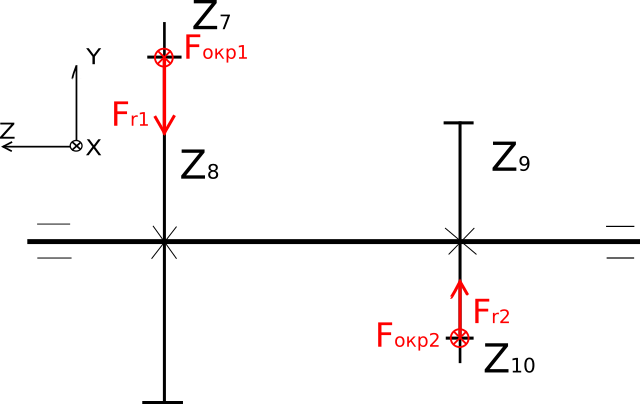
\includegraphics[width=0.7\linewidth]{shaft_schema.png}}
            \caption{Схема вала 4 с приложенными силами}
        \end{figure}
        Найдём необходимые силы (с учётом \( M_4 = 124.27 \)):
        \[ F_{\text{окр1}} = \frac{M_4}{0.5d_1} = 4.69\ H,\]
        \[ F_{\text{окр2}} = \frac{M_4}{0.5d_2} = 11.51\ H,\]
        \[ F_{r1} = F_{\text{окр1}}\cdot tan(20^\cdot) = 1.71\ H,\]
        \[ F_{r2} = F_{\text{окр2}}\cdot tan(20^\cdot) = 4.19\ H,\]

        Найдём реакции в опорах.\par
        \begin{figure}[h]
            \center{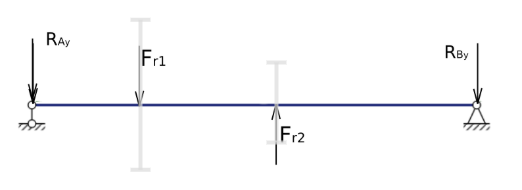
\includegraphics[width=0.8\linewidth]{sh_yoz_2.png}}
            \caption{Схема балки в плоскости YOZ}
        \end{figure}
        \[ \sum M_A = 0 \]
        \[ F_{r_1}\cdot 6 - 15\cdot F_{r_2} + 27\cdot R_{B_y} = 0\]
        \[ R_{B_y} = 1.95\ H\]
        \[ \sum_{i}^{}F_i = 0 \]
        \[ R_{A_y} + F_{r_1} + R_{B_y} = F_{r_2} \]
        \[ R_{A_y} = 0.53\ H\]        
        
        \begin{figure}[h]
            \center{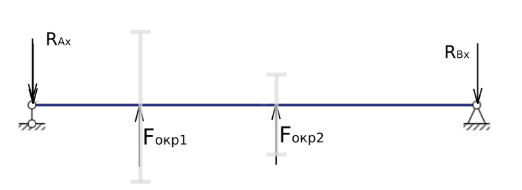
\includegraphics[width=0.8\linewidth]{sh_xoz_2.png}}
            \caption{Схема балки в плоскости XOZ}
        \end{figure}
        \[ \sum M_A = 0 \]
        \[ R_{B_x} = \frac{15\cdot F_{\text{окр2}} + 6\cdot F_{\text{окр1}}}{27} = 7.43\ H\]
        
        \[ R_{A_x} = F_{\text{окр2}} + F_{\text{окр1}} - R_{B_x} = 8.76\ H\]

        Представим эпюры рассчитанных моментов:
 
        \begin{figure}[!h]
            \center{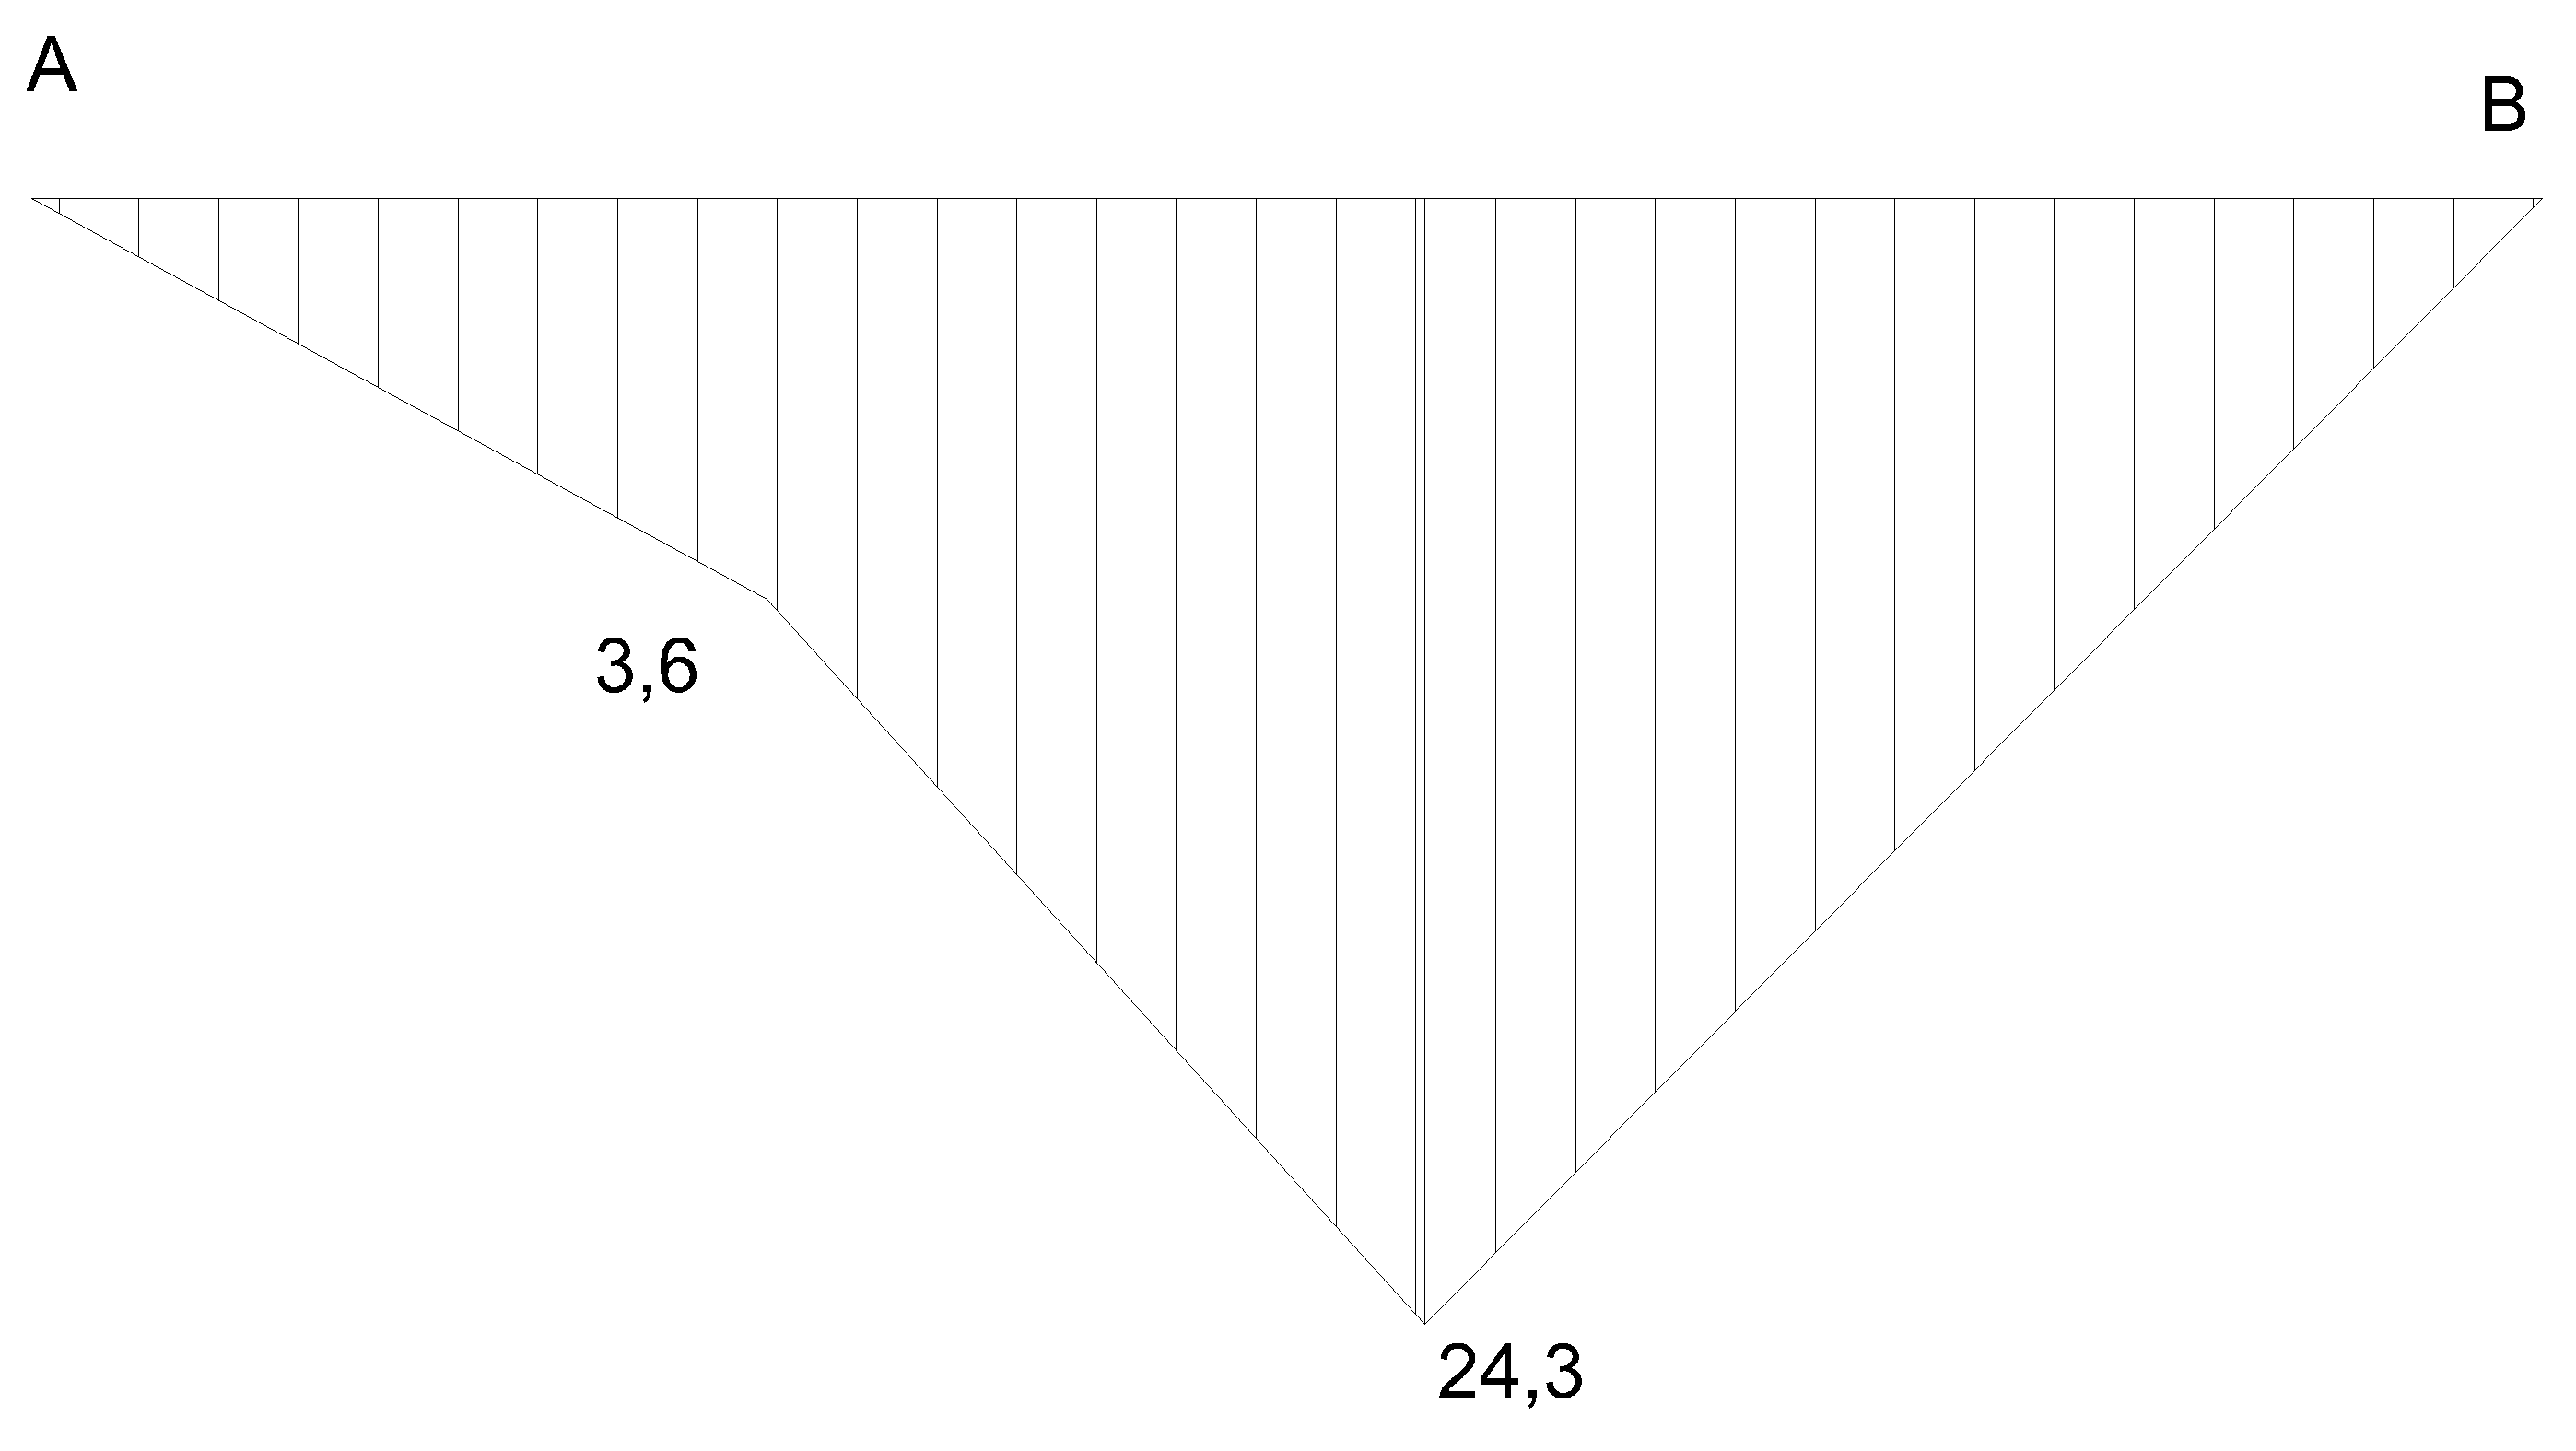
\includegraphics[width=0.8\linewidth]{epure_yoz.png}}
            \caption{Эпюра изгибающего момента в плоскости YOZ}
        \end{figure}

        \begin{figure}[h]
            \center{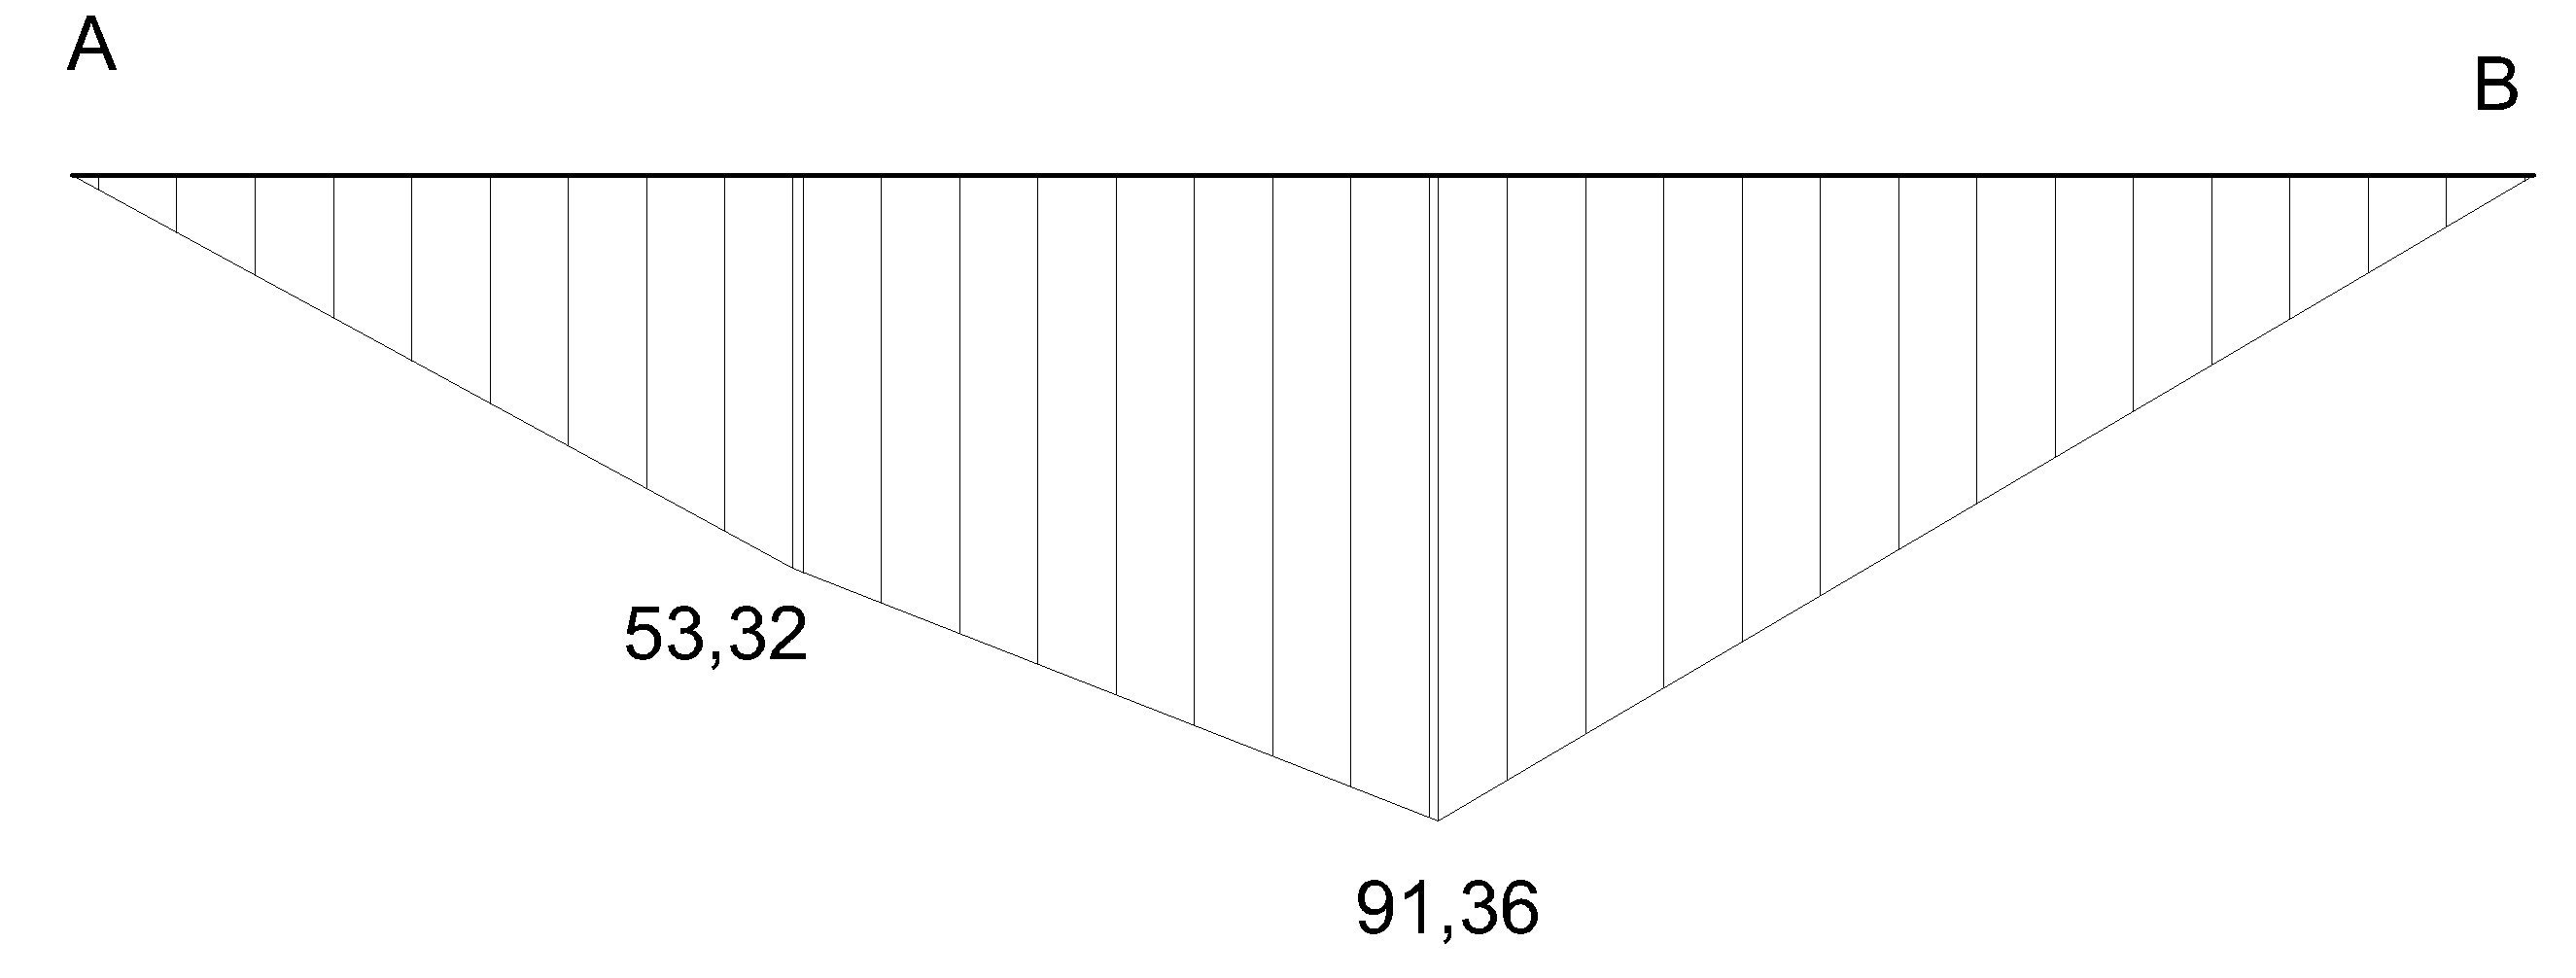
\includegraphics[width=0.8\linewidth]{epure_xoz.png}}
            \caption{Эпюра изгибающего момента в плоскости XOZ}
        \end{figure}
        \begin{figure}[h]
            \center{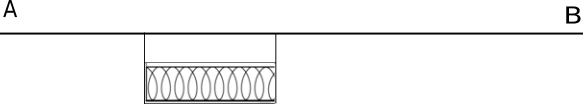
\includegraphics[width=0.8\linewidth]{epure_circ.png}}
            \caption{Эпюра крутящего момента}
        \end{figure}

        Учтя, что на вал действуют одноврененно и изгибающий, и крутящий моменты,
        проведём расчет на прочность через приведенный момент в опасном сечении.
        По эпюрам очевидно, что это сечение находится на месте крепления шестерни
        (зубчатого колеса №9).

        \[ M^{\sum}_\text{изг} = \sqrt{M_x^2 + M_y^2} = \sqrt{91.36^2 + 24.3^2} = 94.54\ \text{Нмм}\]
        \[ M_\text{прив.} = \sqrt{{M^{\sum}_\text{изг}}^2 + 0,75M_\text{кр}^2} = 143.25\ \text{Нмм}\]

        Расчёт минимального диаметра вала проведём по формуле [1]:
        \[ d\geq \sqrt[3]{\frac{M_\text{пр}}{0,1[\sigma_u]}}, \]
        где \( [\sigma_u] \) - допускаемое изгибающее напряжение, вычисляется как
         \( [\sigma_u] = 0,1[\sigma_b] \).\par
        Материалом выберем сталь 40Х, параметры которой приведены в таблице \ref{tab:gear_materials}.\par

        \[ d\geq \sqrt[3]{\frac{143.25}{0,1\cdot 0,1 1000}} = 2.43\ \text{мм} \]
        Принимаем минимальный диаметр ближайшим сверху из стандартных диаметров, равным
        \( d_{\text{мин}} = 3\ \text{мм} \), который при этом вполне подходит по конструктивным
        соображениям. Такой диаметр будет у вала в местах крепления к подшипникам.

    \subsubsection{Расчёт штифтов}
        Расчитаем минимальный диаметр штифта. Для этого воспользуемся следующей формулой:
        \[ d_\text{ш} \geq 2\sqrt{\frac{M}{\pi d [\tau_{\text{ср}}]}}, \]
        где \( [\tau_{\text{ср}}] \) - допустимое напряжение на срез, МПа,\\
        \( d \) - диаметр вала, мм,\\
        \( M \) - крутящий момент на валу, Нмм.
        Материалом для штифта примем Сталь50, для неё \( [\tau_{\text{ср}}] =75\) МПа.
        Так как все валы в местах посадки зубчатых колёс имеют одинаковую толщину d=4мм, то рассчитаем
        толщину штифта для наиболее нагруженного вала V.
        \[ d_\text{ш} \geq 2\sqrt{\frac{121.79}{\pi\cdot 4\cdot 75}} = 0,72\ \text{мм} \]
        Округлив в большую сторону, примем диаметром штифтов \( d_\text{ш} = 1 \) мм.
        

    \subsubsection{Расчёт опор}
        Подберём опоры для валов. Выберем опоры качения, а именно - радиальные подшипники,
        так как нагрузка на валы только радиальная.\par
        Применем формулу для расчёта динамической грузоподьемности [1] (т.к. скорость вращения
        больше 1 об/мин):
        \[ C_P = 0,01P\sqrt[3]{60nL_h}, \]
        где n - частота вращения рассчитываемого вала (IV), об/мин, \\P - эквивалентная
        динамическая нагрузка,\\ \( L_h \) - время работы, ч.\par
        Рассчитаем P по формуле [1]:
        \[ P = (XF_r + YF_a)k_\sigma k_\tau = 10.53\ H, \]
        где (X, Y) = (1, 0) - коэффициенты, учитывающие направление нагрузки,\par
            \( k_\sigma = 1 \) - коэффициент безопасности,\par
            \( k_\tau=1,2 \) - коэффициент температуры,\par
            \( F_r \) - радиальная нагрузка, \par
            \( F_a \) - осевая нагрузка (равна 0).\par
        Приняв n=218 об/мин, \( L_h \) = 3000ч, получаем
        \[ C_P = 0,01\cdot 10.53 \cdot \sqrt[3]{60\cdot 218\cdot 3000} = 35.79\ H \]
        \cite{Dorf}
        На основе полученного значения выберем подшипник "Подшипник шариковый радиальный однорядный №2000083 ГОСТ 8538-74" со следующими
        параметрами:
        \begin{table}[h!]
            \begin{center}
                \begin{tabular}{p{0.13\linewidth}p{0.13\linewidth}p{0.13\linewidth}p{0.13\linewidth}p{0.13\linewidth}p{0.13\linewidth}}
                    \hline
                    d, \( \text{мм} \) & D, \( \text{мм} \) & B, \( \text{мм} \) & r, \( \text{мм} \) & C, Н & \( C_0 \), Н \\
                    \hline
                    3 & 7 & 2.5 & 0.3 & 430 & 136 \\
                    \hline
                \end{tabular}
                \caption{{Характеристики основного подшипника}}\label{tab:podsh}
            \end{center}
        \end{table}

        Выберем такой подшипник для всех валов.
        

        
        
        
        
        
        
        
        

        
        
\newpage
        ferefr
\renewcommand\refname{Список использованных источников}
\addcontentsline{toc}{section}{4. Список использованных источников}
\bibliographystyle{utf8gost705u}  %% стилевой файл для оформления по ГОСТу
\bibliography{biblio}
        
[1] Тищенко \par
[2] Шарловский
    
\end{document}